% !TEX TS-program = pdflatex
% !TEX encoding = UTF-8 Unicode

% This is a simple template for a LaTeX document using the "article" class.
% See "book", "report", "letter" for other types of document.

\documentclass[11pt]{article} % use larger type; default would be 10pt

\usepackage[utf8]{inputenc} % set input encoding (not needed with XeLaTeX)
\usepackage{graphicx}
\usepackage{algorithm}
\usepackage{algorithmicx}
\usepackage{algpseudocode}
\usepackage{multirow}

%%% Examples of Article customizations
% These packages are optional, depending whether you want the features they provide.
% See the LaTeX Companion or other references for full information.

%%% PAGE DIMENSIONS
\usepackage{geometry} % to change the page dimensions
\geometry{a4paper} % or letterpaper (US) or a5paper or....
% \geometry{margin=2in} % for example, change the margins to 2 inches all round
% \geometry{landscape} % set up the page for landscape
%   read geometry.pdf for detailed page layout information

\usepackage{graphicx} % support the \includegraphics command and options

% \usepackage[parfill]{parskip} % Activate to begin paragraphs with an empty line rather than an indent

%%% PACKAGES
\usepackage{booktabs} % for much better looking tables
\usepackage{array} % for better arrays (eg matrices) in maths
\usepackage{paralist} % very flexible & customisable lists (eg. enumerate/itemize, etc.)
\usepackage{verbatim} % adds environment for commenting out blocks of text & for better verbatim
\usepackage{subfig} % make it possible to include more than one captioned figure/table in a single float
% These packages are all incorporated in the memoir class to one degree or another...

%%% HEADERS & FOOTERS
\usepackage{fancyhdr} % This should be set AFTER setting up the page geometry
\pagestyle{fancy} % options: empty , plain , fancy
\renewcommand{\headrulewidth}{0pt} % customise the layout...
\lhead{}\chead{}\rhead{}
\lfoot{}\cfoot{\thepage}\rfoot{}

%%% SECTION TITLE APPEARANCE
\usepackage{sectsty}
\allsectionsfont{\sffamily\mdseries\upshape} % (See the fntguide.pdf for font help)
% (This matches ConTeXt defaults)

%%% ToC (table of contents) APPEARANCE
\usepackage[nottoc,notlof,notlot]{tocbibind} % Put the bibliography in the ToC
\usepackage[titles,subfigure]{tocloft} % Alter the style of the Table of Contents
\renewcommand{\cftsecfont}{\rmfamily\mdseries\upshape}
\renewcommand{\cftsecpagefont}{\rmfamily\mdseries\upshape} % No bold!

%%% END Article customizations

%%% The "real" document content comes below...

\title{Lab 4: Dimensionality Reduction}
\author{Ruofan Zhou}
%\date{} % Activate to display a given date or no date (if empty),
         % otherwise the current date is printed 

\begin{document}
\maketitle

\section{Faces}
1. Done\\
2.  The eignvalue plot is as below:\\
\centerline{
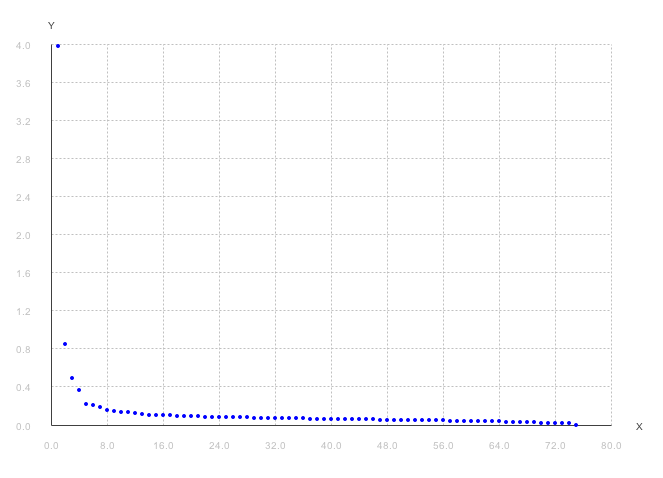
\includegraphics[width=13cm]{pic/p4}}\\
3. I think that the faces have \emph{7} features: \emph{mouth radian, eyes size, eyes color, hair length, hair color, face color and hat color}.\\
4. I sorted the variances and get the plot: \\
\centerline{
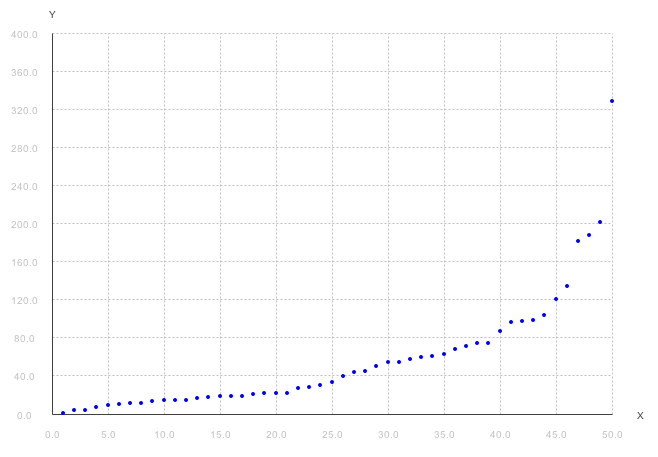
\includegraphics[width=13cm]{pic/p2}}\\
but still can't really find how many dimensions it can be precised to.\\
5. It's really hard and I give it up.\\

\subsection{Principal Component Analysis}
6. Done.\\
7. See the plot of the variances as below. It's obvious that \emph{7} components are stand out, and it's equal to the answer of quesion 2.\\
\centerline{
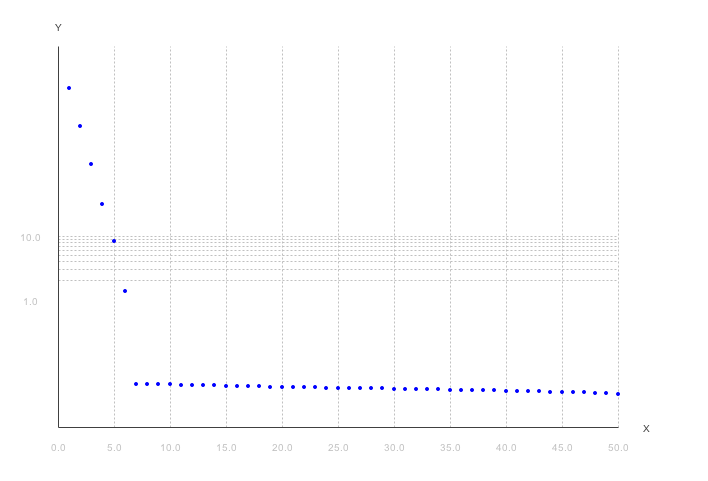
\includegraphics[width=10cm]{pic/p3}}
8. \& 9. Done. And it seems that the correspondence between principal components and facial features are as below:
\begin{table}[!hbp]
\centering
\begin{tabular}{|c|c|}
\hline
Principal Component & Facial Feature \\
\hline
dim1 & mouth radian\\
\hline
dim2 & eyes size \\
\hline
dim3 & eyes color \\
\hline
dim4 & hair length \\
\hline
dim5 & hair color \\
\hline
dim6 & face color \\
\hline
dim7 & hat color \\
\hline
\end{tabular}
\end{table}\\
10. With very happy(mouth up) face[dim 1], whose eyes are slightly larger than normal[dim 2] and green[dim 3]. His hair is relatively short[dim 4] and is in bright yellow color[dim 5]. Normal face color(not too dark or too bright)[dim 6], and pobably with a brown hat[dim 7].\\

\section{Smartvote}
1.  Done.\\
2.  See the \emph{variance-dimension} plot as below:\\
\centerline{
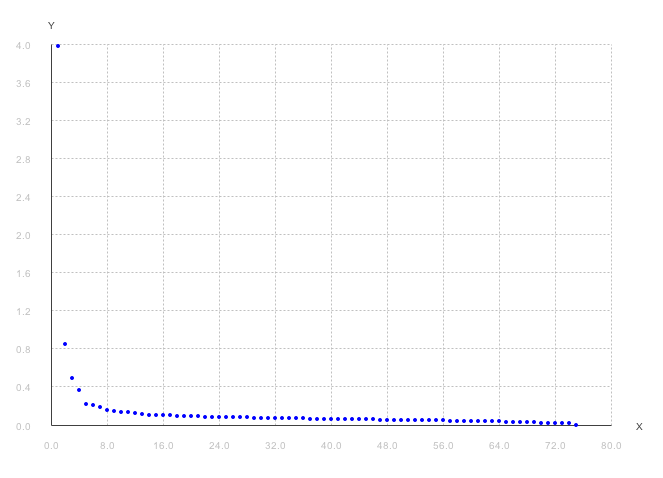
\includegraphics[width=13cm]{pic/p4}}\\
3.  The first principal component exlain \emph{0.378182} of the variance; the first two principal components exlain \emph{0.458936} of the variance; the first three principal components exlain \emph{0.505655} of the variance.\\
4.  The plot is as below: \\
\centerline{
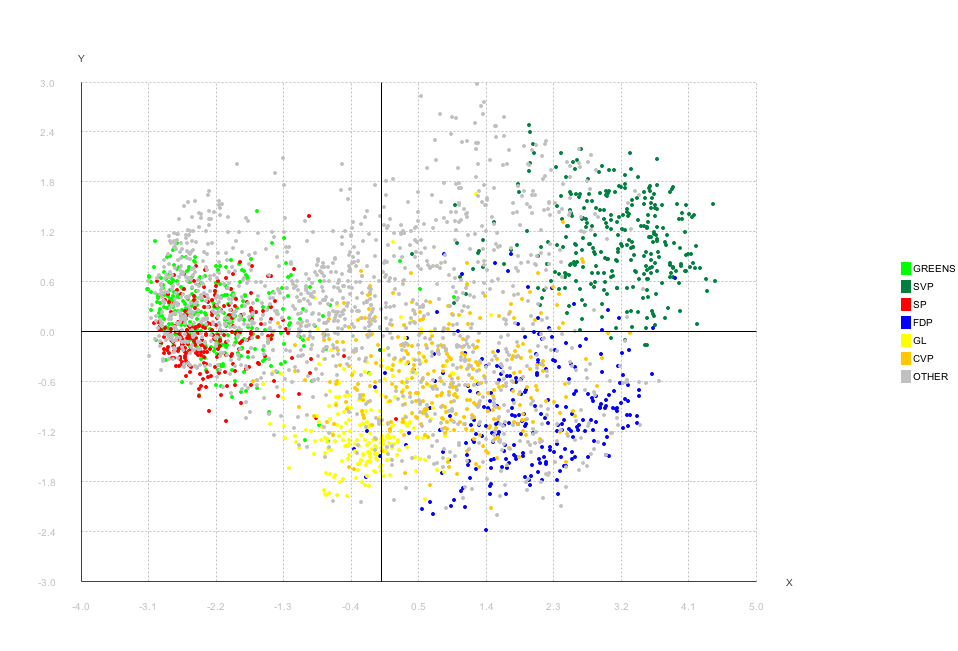
\includegraphics[width=13cm]{pic/p5}}\\
5.  The x-axis shows the \emph{political ideas} (i.e., nagetive value is authoritarianism, while the positive ones are libertarianism);  The y-axis shows the \emph{social and cultural concepts} (i.e., nagetive value is conservatism, while the positive ones are lliberalism). While the first principal direction is correspondented to the x-axis and the second to the y-axis.\\
6.  Maybe the \emph{economic concepts}? (i.e., nagetive value is communisum, while the positive ones are neoliberalism, I'm not sure, I'm not good at political:( )\\
7.  I find the most relevent questions by \emph{find the maximum absolute value of the coressponding column}. And the most relevant questions I think is showed as below:\\
\emph{First Component:}\\
Would you support foreigners who have lived for at least ten years in Switzerland being given voting and electoral rights at municipal level throughout Switzerland?\\
Would you essentially welcome greater restriction on the tax competition that applies between the cantons?\\
A recently launched popular initiative is proposing to limit the maximum salary that can be earned in a company to 12 times the lowest salary (the "1:12" initiative). Do you support this idea?\\
\emph{Second Component:}\\
Today, the Swiss Army can take part in UN or OSCE peace-keeping missions abroad, armed for self-defence purposes. Do you approve?\\
Should Switzerland conclude an agricultural free trade agreement with the EU?\\
Do you support the existing agreement with the EU on the free movement of peoples?\\
\emph{Third Component:}\\
Would you support the right of doctors in Switzerland to help someone die with impunity?\\
Should same-sex couples who have registered their partnership be able to adopt children?\\
Switzerland has relatively strict rules when it comes to medically assisted reproduction. Should these be relaxed?\\
8. The number of the questions is a little large. But I think that the "relevent quetions" achieved in step 7 is quite correct. \\
\end{document}
